\documentclass[12pt, dvipdfmx]{jsbook}
\usepackage{amsmath,amssymb,bm}
\usepackage{subfigure}
\usepackage{minitoc}
\usepackage{hhline}
\usepackage{diagbox}
\usepackage{booktabs}
\usepackage{comment}
\usepackage{ulem}
\usepackage{url}
\usepackage{color}
\usepackage{latexsym}
\usepackage{ascmac}
\usepackage{subfig}
\usepackage[labelsep=quad]{caption}
\usepackage{./sty/bthesis}
\usepackage{./sty/xbmkanji}
\usepackage{./sty/cite}
\usepackage{./sty/algorithm}
\usepackage{./sty/algorithmic}

\renewcommand\UrlFont{\rmfamily}
\renewcommand{\refname}{}

\newcommand\whline{%
     \noalign{\xdef\origarrayrulewidth{\the\arrayrulewidth}%
     \global\arrayrulewidth 3\arrayrulewidth}%
     \hline%
     \noalign{\global\arrayrulewidth\origarrayrulewidth}%
}

%%%%%%%%%%%%%%%%%%%%%%%%%%%%%%%%%%%%%%%%
\newif\iffigure
%\igurefalse
\figuretrue
%%%%%%%%%%%%%%%%%%%%%%%%%%%%%%%%%%%%%%%%

%\setlength{\subfigtopskip}{-10pt}
%\setlength{\subfigcapskip}{-10pt}
%\setlength{\subfigbottomskip}{-10pt}
%\setlength{\abovecaptionskip}{-10pt}
%\setlength{\belowcaptionskip}{-10pt}

%
% 論文の表紙の項目
%
\thesistype{令和元年度 卒業論文}
\title{土砂自動積み込みのための\\画像認識と点群位置合わせによる\\ダンプトラックの位置姿勢推定}
\etitle{Dump Truck Position and Posture Estimation \\by Image Recognition and Point Cloud Registration\\ for Automatic Loading}
\affiliation{千葉工業大学 先進工学部 未来ロボティクス学科}
\supervisor{藤井 浩光\ \ 准教授}
\studentid{16C1101}
\author{畠山 佑太}
\begin{document}
\dominitoc
%表紙
\maketitle
%概要
\thispagestyle{empty}
\thispagestyle{empty}
\chapter*{概要}
\markboth{概要}{}
\label{abst}
\def\thepage{}
\thispagestyle{empty}



\thispagestyle{empty}

\newpage
%%%%%%%%%%%%%%%%%%%%%%%%%%%%%%%%%%%%%%%%%%%%%%%%%%%%%%%%%%%%%%%%%%%%%%%%%%%%%%%

%%%%%%%%%%%%%%%%%%%%%%%%%%%%%%%%%%%%%%%%%%%%%%%%%%%%%%%%%%%%%%%%%%%%%%%%%%%%%%%
%%% Local Variables:
%%% mode: katex
%%% TeX-master: "../thesis"
%%% End:


\frontmatter
%目次
\tableofcontents
%図目次
\listoffigures
%表目次
\listoftables

%
%以下本文
\mainmatter
%========================================
% コンパイルはどんどん重くなっていくので
% 執筆を進める上では必要な部分だけを
% コメントアウトしてコンパイルすると良い
%========================================
\chapter{序論}
\thispagestyle{empty}
\label{Chap1}
\minitoc

\newpage
%%%%%%%%%%%%%%%%%%%%%%%%%%%%%%%%%%%%%%%%%%%%%%%%%%%%%%%%%%%%%%%%%%%%%%%%%%%%%%%

%==============================================================================
%背景
%==============================================================================
\section{背景}
\label{Background}
建設業は,道路、河川などの社会資本や産業施設,公共施設の整備・維持管理を行い,国内総生産及び就業者数の約10%を占める基幹産業の一つである.\cite{日本建設組合連合2016}
\par 2010 年に発生した東日本大震災や各地の豪雨災害時での復興活動などで,建設業の重要性が再認識されている.
しかし,近年の建設業界では,技能労働者の高齢化や就業者の減少により熟練オペレーター不足が問題となってい
る.また,国土交通省の「建築産業の現状と課題」\cite{建設経済研究所2017}によると,2015 年の技能労働者数は330 万人であり,10 年後
の 2025 年は 286 万人と減少すると試算されている.今後,深刻な人材不足の危機に陥ると予想されており,人材不
足を補う為,建設現場における作業の自動化は重要な課題である.
\par
現場における作業で自動化の要求の高い作業の一つが,バックホウとダンプトラックの連携による土砂積み込み作業の自動化である.
土砂の積み込みの際には,ダンプトラックは運転手により積み込み可能な位置まで移動されるが,バックホウによる積み込み作業を自動化するために
は,バックホウに対するダンプトラックの相対的な位置姿勢を正しく獲得する必要がある.
一般の作業現場では,GNSSやTotal Stationによって位置姿勢の把握\cite{土井下2010}が行われているが,GNSS等の衛星測位システムで高精度な位置姿勢を獲得するためには,通信基地局などの環境整備が必要であり,設備コストが大きいことが課題である.
Tostal Stationは建機に搭載されたプリズムにレーザーを照射することで高精度な位置情報を獲得できるが,一旦,レーザー照射が途切れるとプリズムを
追従できない問題がある.
そのため,環境に大がかりな設備を要さずに位置姿勢を計測する手法が期待されている.
%%%%%
\begin{figure}[b]
 \begin{center}
 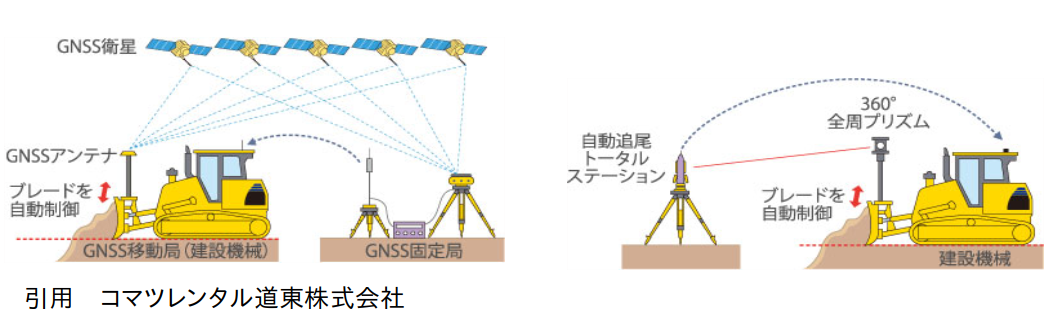
\includegraphics[width=1.0\columnwidth]{./chap1/fig/GNSS.png}
 \caption{GNSSやTSによる位置情報の把握}
 \label{fig:GNSS}
 \end{center}
 %\vspace{-5mm}
\end{figure}
%%%%%

\newpage

\section{従来研究}
対象物体にセンサを搭載せずに外部からのセンシングによる位置姿勢推定の手法が研究されており,マニピュレータによるピッキング作業のための物体検出や
自動運転ための車両の検出などを目的とした研究が多くされている.

ピッキング作業ための物体検出として,RGB-Dセンサの計測結果と対象物体のCADモデルとの照合による3次元物体計測が検討されてきた.\cite{中原智治2001}\cite{林2008}\cite{西卓郎2014}
また近年では深層学習を取り入れたアプローチも増えており,対象物体のあらゆる姿勢の画像をCADデータから生成したものを教師データとした深層学習による推定手法\cite{Sundermeyer2018}\cite{Tremblay2018}などがある.
しかし,実際の作業現場では様々なメーカーのダンプトラックが行き交い,また荷台部も現場によって異なるため,事前にCADデータを用意するのは難しい.

また,車両を対象とした位置姿勢推定の手法としてLIDARを用いた3次元物体検出がある.\cite{Zhang2017}\cite{Chen2017}\cite{Lang2019}\\
図のように広域にレーザーを照射することにより計測した3次元点群から対象物体の点群を検出することで位置姿勢推定を行う.
しかし,土砂積み込み作業は高低差がある環境が多く,LIDARは視野角が狭いため近距離が死角になる.また,LIDARを傾けることで死角を
減らせるが,距離によっては対象物体にレーザー当たらず計測ができない状況が生じる.

\newpage
\section{研究の目的}
1.1 節で述べたように,環境に大がかりな設備を要せずにダンプトラックの位置姿勢を計測する手法が求められている.
そのため,Cバックホウに搭載したRGB-Dセンサから得られるダンプトラックの3次元データを用いた点群位置合わせに基づく位置姿勢推定が有効だと考えられる.
しかし,RGB-Dセンサは点群位置合わせを行う上で有効な高密度の3次元点群を得られるが,計測距離が短く計測できる範囲は狭く,
実際の土砂積み込み作業の際は,ダンプトラックは遠方からバックホウに向かって進入してくる場合が多く,ダンプトラックの進入を判断するためには,
遠方にあるダンプトラックの存在とその大まかな位置姿勢を計測する必要がある.



\par
そこで,本研究では
    \begin{screen}
        \begin{center}
        計測範囲の拡張と距離センサの計測範囲外でも計測可能なダンプトラックの位置姿勢推定手法の提案
        \end{center}
    \end{screen}
を目的とする
\newpage
\section{本論文の構成}
本論文は全4章から構成されている.図に本論文の構成を示す.\par
第1章では,本研究の背景,従来研究,目的について述べた.\par
第2章では,画像認識と点群位置合わせによるダンプトラックの位置姿勢推定の提案手法について述べる.\par
第3章では,本提案手法の有効性を検証するために行った実験について述べる.\par
第4章では,結論と今後の展望を述べる.
\begin{figure}[b]
    \begin{center}
    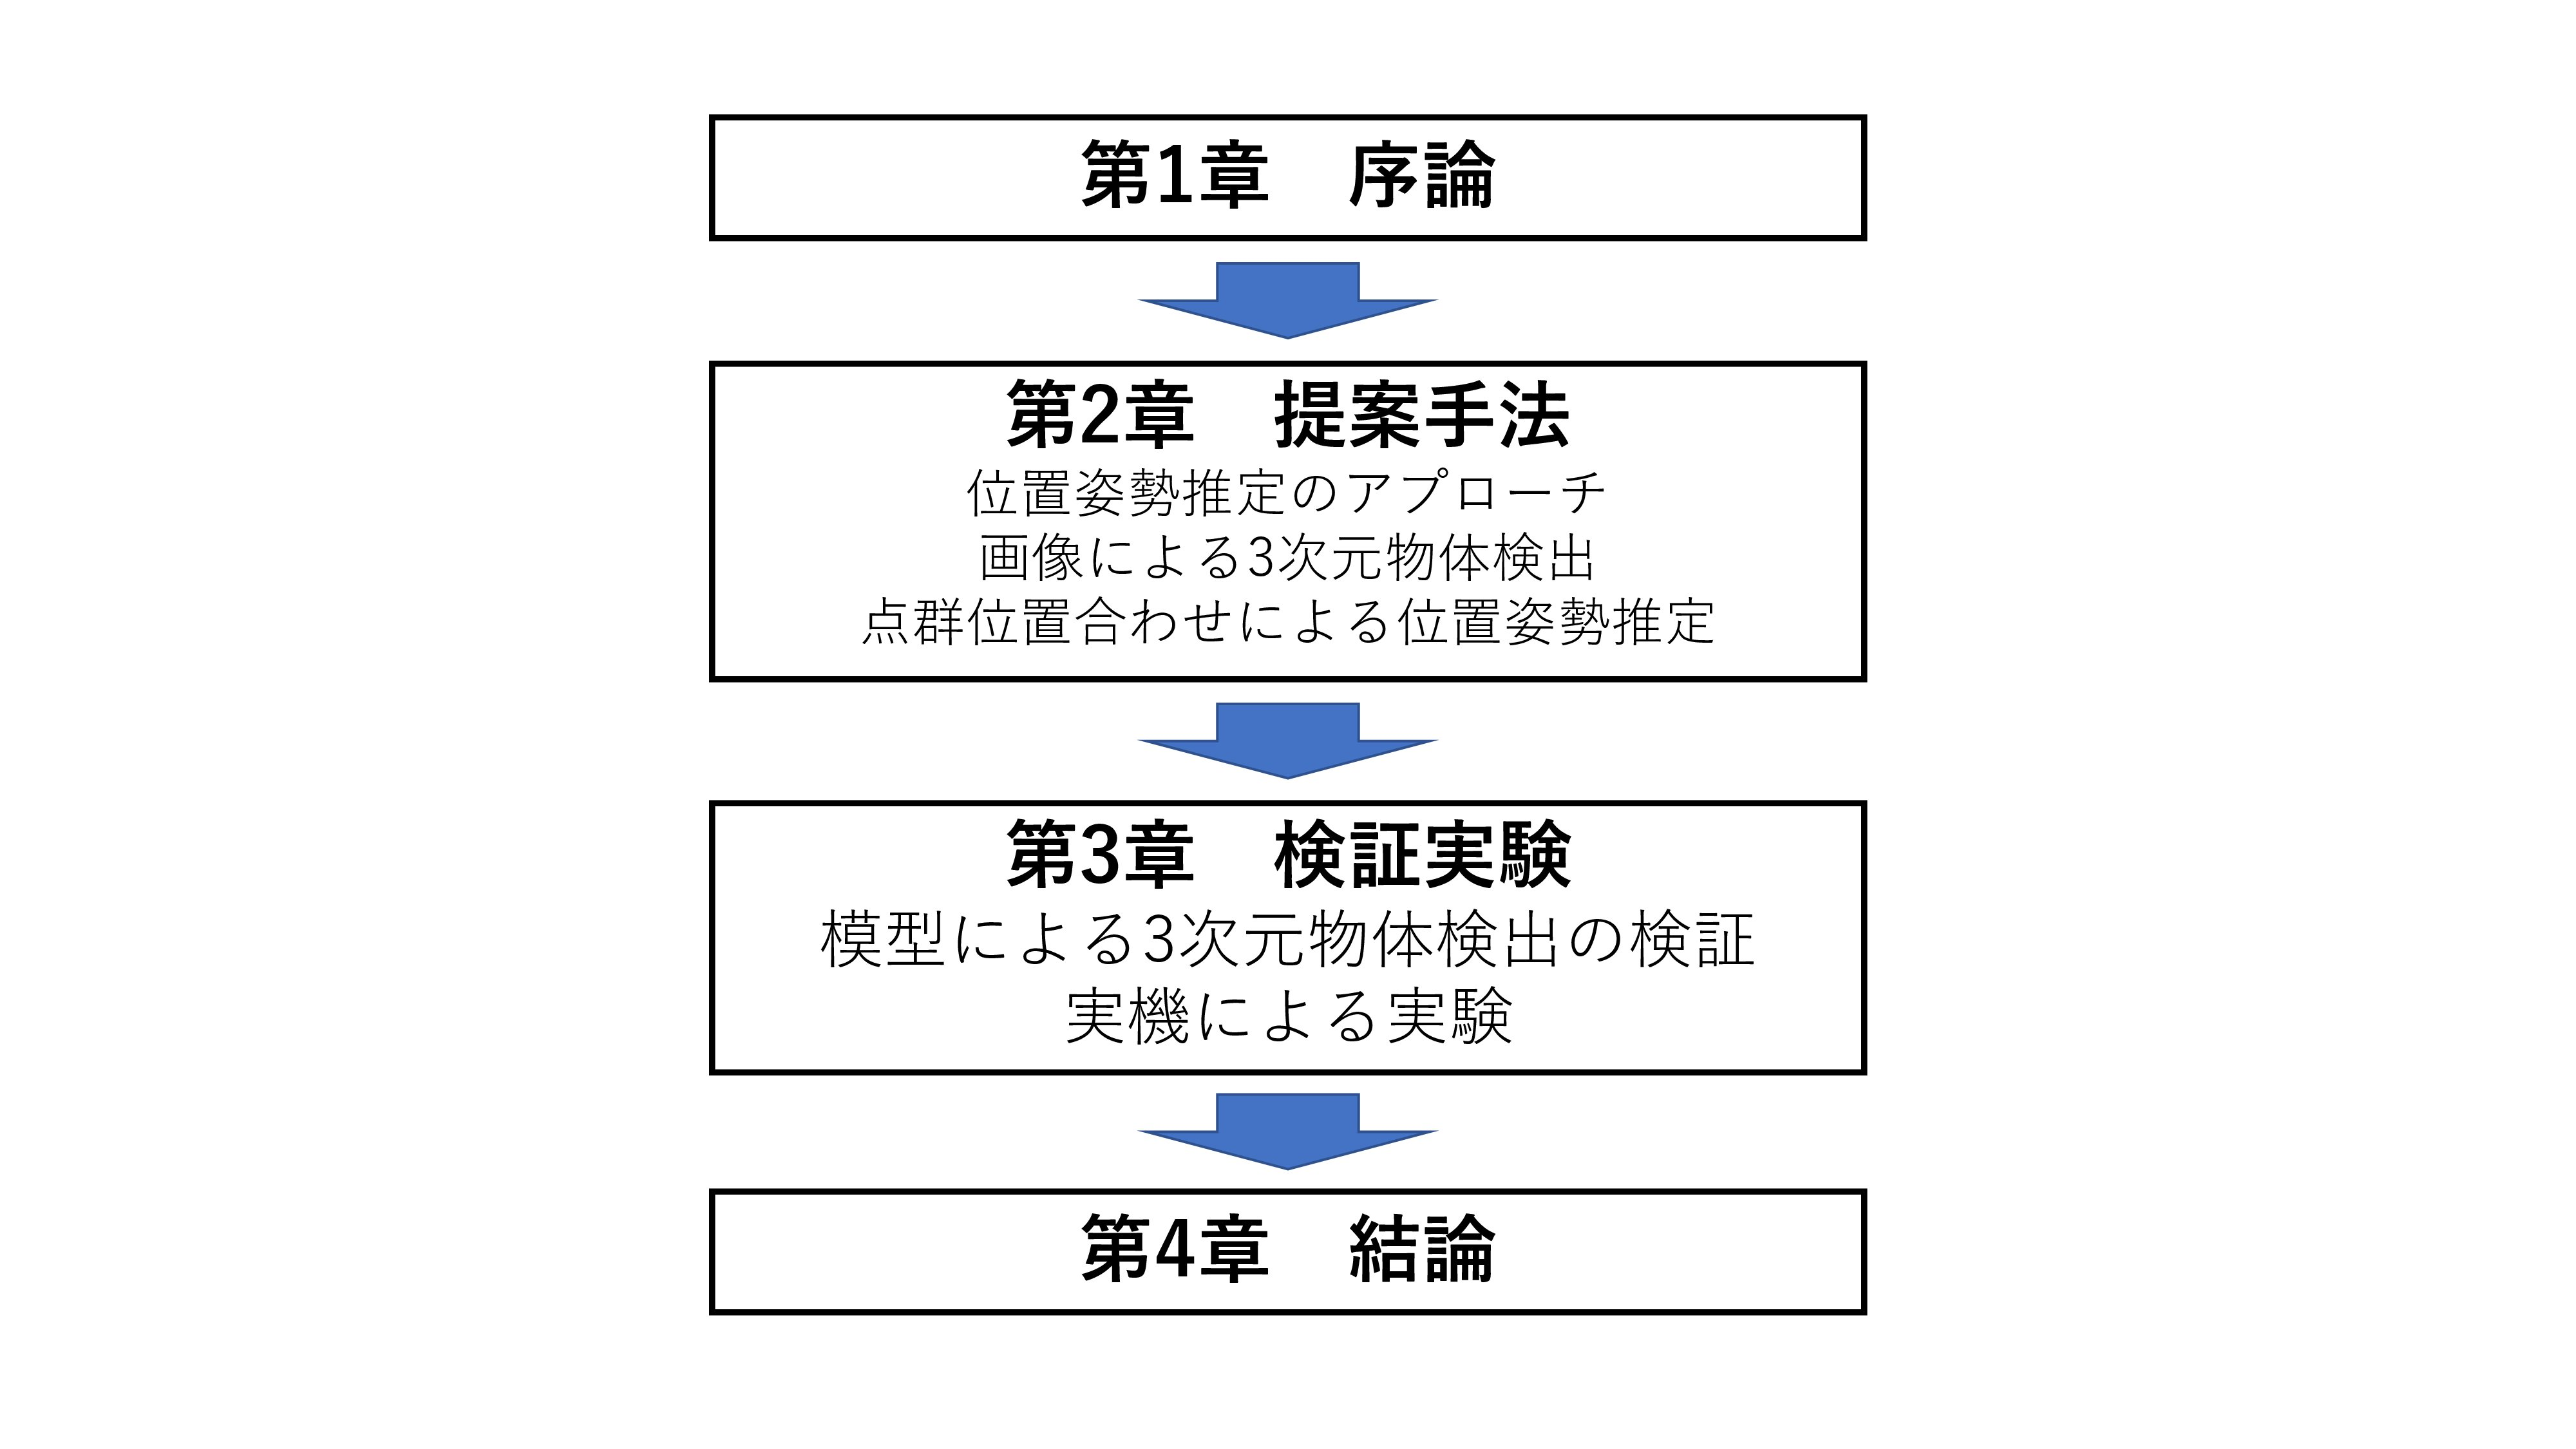
\includegraphics[width=0.3 \columnwidth]{./chap1/fig/struct.jpg}
    \caption{本論文の構成}
    \label{fig:flow}
    \end{center}
    %\vspace{-5mm}
   \end{figure}

%%%%%%%%%%%%%%%%%%%%%%%%%%%%%%%%%%%%%%%%%%%%%%%%%%%%%%%%%%%%%%%%%%%%%%%%%%%%%%%
%%% Local Variables:
%%% mode: katex
%%% TeX-master: "../thesis"
%%% End:
\chapter{提案手法}
\thispagestyle{empty}
\label{chap2}
\minitoc

\newpage
%%%%%%%%%%%%%%%%%%%%%%%%%%%%%%%%%%%%%%%%%%%%%%%%%%%%%%%%%%%%%%%%%%%%%%%%%%%%%%%
%==============================================================================
%はじめに
%==============================================================================
\section{はじめに}
本章では,画像による3次元物体検出と点群位置合わせによるダンプトラックの位置姿勢推定をするための手法について述べる.
\par
2.2 節では,ダンプトラックの位置姿勢を推定するために画像による3次元物体と点群位置合わせを統合したダンプトラックの位置姿勢推定のアプローチについて述べる.
\par
2.3 節では,画像による3次元物体検出の手法について述べる.
\par
2.4 節では,点群位置合わせによるダンプトラックの位置姿勢推定について述べる.
\newpage

\section{位置姿勢推定のアプローチ}
\subsection{画像による3次元物体検出と点群位置合わせによる位置姿勢の概要}
第 1 章で述べたように本研究ではダンプトラックの位置姿勢を計測するために画像による3次元物体検出と点群位置合わせを統合した位置姿勢推定の手法を用いる.
その概要について説明する.
\par
事前に点群位置合わせの基準となるダンプトラックの3次元モデルを作成を行う.バックホウに搭載した複数台のRGB-Dセンサから土砂積み込み作業範囲に
設置したダンプトラックを計測し3次元点群を取得する.取得した3次元点群は地面情報やノイズを含むためダンプトラックの点群を抽出することで3次元モデルを作成する.
\par
次に位置姿勢推定の概要について説明する.
ダンプトラックは土砂積み込み作業範囲外からバックホウに向かって進入すると仮定し,バックホウに向かって進入するダンプトラックを
バックホウに搭載したRGB-Dセンサから撮影し,画像による3次元物体検出を行う.推定値が土砂積み込み作業範囲外であれば3次元物体検出を続けて行い,
範囲内であれば,推定値を初期値として入力を行い,計測した3次元点群と事前に作成した3次元モデルとの点群位置合わせにより位置姿勢推定を行う.
また,3次元物体検出はダンプトラックが映っているのにかかわらず未検出となる場合ある.未検出の際は前フレームを参照し,ダンプトラックの位置が土砂積み込み
作業範囲内であれば3次元特徴量マッチングを初期値とした点群位置合わせにより位置姿勢推定を行う.
\newpage
\subsection{位置姿勢推定システムの概要}
本節では,画像による3次元物体検出や点群位置姿勢に必要となる画像や点群を計測する方法を説明する.

\newpage
\section{画像による3次元物体検出}
\subsection{深層学習による3次元物体検出}
\newpage
\subsection{データセットの作成}

\section{点群位置合わせによる位置姿勢推定}
\subsection{ダンプトラックの点群抽出}
\subsection{点群位置合わせ}
\subsection{3次元特徴量マッチング}
\section{おわりに}

%\chapter{検証実験}
\thispagestyle{empty}
\label{chap3}
\minitoc

\newpage
%%%%%%%%%%%%%%%%%%%%%%%%%%%%%%%%%%%%%%%%%%%%%%%%%%%%%%%%%%%%%%%%%%%%%%%%%%%%%%%
%==============================================================================
%はじめに
%==============================================================================
\section{はじめに}
本章では,第 2 章で述べた提案手法の有効性を検証するために行った実験について述
べる.
\par
3.2 では,模型による3次元物体検出の実験と結果について述べる.
\par
3.3 では,実機による実験に使用した装置の構成,計測対象,実験方法について述べる.
\par
3.4 では,提案手法による処理結果,位置姿勢推定の結果について述べる.
\newpage

\section{模型による3次元物体検出の実験}
\subsection{実験環境}
本節では,模型による3次元物体検出の実験に使用したデータセットの作成環境と実験方法について述べる.図\ref{fig:tr}に示すように,データセットの作成には,回転台,ダンプトラックの模型とRGB-Dを使用した.
回転台は,ComXimのターンテーブル(\ref{fig:table}),ダンプトラックの模型(\ref{fig:truck})は,プラッツの1/50日野プロフィア(\ref{tab:truck}),RGB-Dセンサは,IntelのRealSense D435i(\ref{tab:intel}) を使用した.表\ref{tab:table},
表\ref{tab:truck},表\ref{tab:intel}
にそれぞれ,回転台,模型とRGB-Dセンサの仕様を示す.RGB-Dセンサは,内蔵したIMUにより取得した姿勢を基に地面に並行となるようにセンサ座標を座標変換する.
\begin{figure}[b]
    \begin{center}
    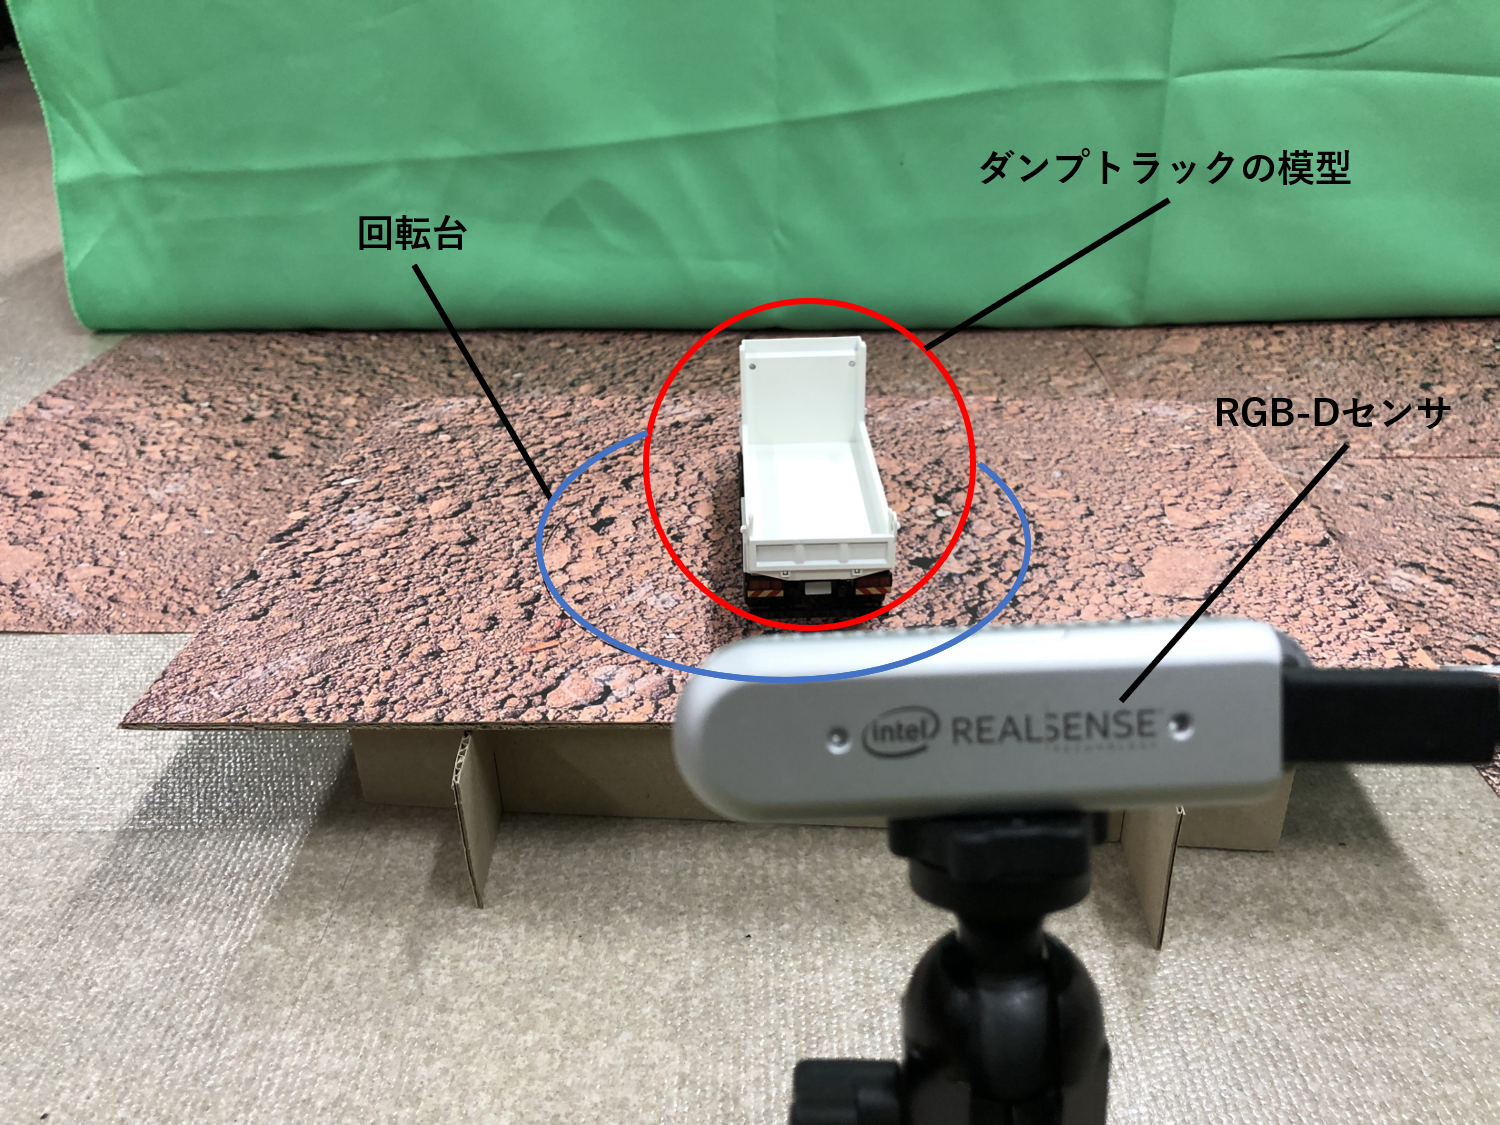
\includegraphics[width=0.5\columnwidth]{./chap3/fig/train.eps}
    \caption{撮影環境}
    \label{fig:tr}
    \end{center}
    %\vspace{-5mm}
\end{figure}

\begin{figure}[b]
    \begin{minipage}{0.5\hsize}
     \begin{center}
      \includegraphics[width=45mm]{./chap3/fig/table.eps}
     \end{center}
     \caption{ComXim ターンテーブル}
     \label{fig:table}
    \end{minipage}
    \begin{minipage}{0.5\hsize}

    \begin{center}
     \includegraphics[width=45mm]{./chap3/fig/truck.eps}
    \end{center}
     \caption{プラッツ 1/50日野プロフィア}
     \label{fig:truck}
    \end{minipage}
    
\end{figure}
\clearpage

\begin{figure}[b]
    \begin{center}
    \includegraphics[width=0.4\columnwidth]{./chap3/fig/intel.eps}
    \caption{IntelのRealSense D435i}
    \label{fig:intel}
    \end{center}
    %\vspace{-5mm}
\end{figure}

\begin{table}[b]
    \begin{center}
    \caption{ComXim ターンテーブル}
    \begin{tabular}{|c|c|}
    \hline
    最大耐荷重     & 20 kg   \\ \hline
    角度分解能     & 0.1 deg \\ \hline
    外形寸法(R x H) & 20 x 5 cm \\ \hline
    質量        & 0.8 kg  \\ \hline
       \end{tabular}
    \label{tab:table}
    \end{center}
\end{table}

\begin{table}[b]
    \begin{center}
    \caption{プラッツ 1/50日野プロフィア}
    \begin{tabular}{|c|c|}
    \hline
    外形寸法(L x W x H) & 160 x 60 x 71 mm \\ \hline
    質量          & 281 g        \\ \hline
    \end{tabular}
    \label{tab:truck}
    \end{center}
\end{table}

\begin{table}[b]
    \begin{center}
    \caption{Intel RealSense D435i}        
\begin{tabular}{|c|c|}
\hline
解像度(W x H)      & 1280 x 720               \\ \hline
動作範囲      & 0.1 $\sim$ 10 m            \\ \hline
Depth 視野角 & 87° x 58° x 95° \\ \hline
RGB 視野角   & 69° x 42° x 77°      \\ \hline
IMU       & BMI055                   \\ \hline
    \end{tabular}
    \label{tab:intel}
    \end{center}
\end{table}

\clearpage

\subsection{検証結果}
\section{実機による実験}
\subsection{実験環境}
\subsection{実験方法}
\section{実機による実験の結果}
\subsection{ダンプトラックの点群抽出の結果}
\subsection{位置姿勢推定の結果}
\section{おわりに}

%\chapter{結論}
\thispagestyle{empty}
\label{chap4}
\minitoc

\newpage
%%%%%%%%%%%%%%%%%%%%%%%%%%%%%%%%%%%%%%%%%%%%%%%%%%%%%%%%%%%%%%%%%%%%%%%%%%%%%%%
%==============================================================================
%はじめに
%==============================================================================
\section{まとめ}
\section{今後の展望}
%\chapter{結論}
\thispagestyle{empty}
\label{chap5}
\minitoc

\newpage
%%%%%%%%%%%%%%%%%%%%%%%%%%%%%%%%%%%%%%%%%%%%%%%%%%%%%%%%%%%%%%%%%%%%%%%%%%%%%%%
%==============================================================================
%はじめに
%==============================================================================
\section{まとめ}
\section{今後の展望}


%\input{./chap6/chap6}
%\input{./chap7/chap7}
\cleardoublepage
%
%謝辞
\addcontentsline{toc}{chapter}{謝辞}
\chapter*{謝辞}
\thispagestyle{empty}
\markboth{謝辞}{}
\label{thankyou}
%\def\thepage{}

\newpage

本研究を進めるにあたり,ご指導,ご協力をいただいた方々に,
この場をお借りし深く感謝申し上げます.
\\

\begin{flushright}
令和元年 2月 千葉工太郎
\end{flushright}


\newpage
%%%%%%%%%%%%%%%%%%%%%%%%%%%%%%%%%%%%%%%%%%%%%%%%%%%%%%%%%%%%%%%%%%%%%%%%%%%%%%%

%%%%%%%%%%%%%%%%%%%%%%%%%%%%%%%%%%%%%%%%%%%%%%%%%%%%%%%%%%%%%%%%%%%%%%%%%%%%%%%
%%% Local Variables:
%%% mode: katex
%%% TeX-master: "../thesis"
%%% End:

\cleardoublepage
%	
%参考文献
\addcontentsline{toc}{chapter}{参考文献}
\chapter*{参考文献}
%\addcontentsline{toc}{chapter}{参考文献}
\lhead[参考文献]{}
%\renewcommand{\refname}{引用文献}
\thispagestyle{empty}

\newpage

%==============================================================================
%和文文献
%==============================================================================
\subsection*{\textmc{<和文文献>}}
\begin{mythebibliography}{}



\bibitem[建設経済研究所 2017]{建設経済研究所2017}
\leavevmode \\建設経済研究所:
\newblock ``建築産業の現状と課題'',
\newblock 建設経済レポート, Vol.~69, pp.~182--213, 2017.
\\
\bibitem[国土交通省 2015]{国土交通省2015}
\leavevmode \\国土交通省:
\newblock ``建設業'',
\newblock http://www.mlit.go.jp/common/001191669.pdf, 2015, 閲覧日~2019.12.24.
\\
\bibitem[土井下 2010]{土井下2010}
\leavevmode \\土井下~健治, 村本~英一, 神田~俊彦:
\newblock ``建設機械へのICT応用'',
\newblock Komatsu Technical Report, Vol.~56, No.~163, 2010.
\\
\newpage

\bibitem[中原智治 2001]{中原智治2001}
\leavevmode \\中原智治,顧海松,荒木秀和,藤井裕之:
\newblock ``3次元認識によるビンピッキングシステムの実用化'',
\newblock システム制御情報学会論文誌, Vol.~14, No.~4, pp.~226--232, 2001.
\\
\bibitem[林 2008]{林2008}
\leavevmode \\林俊寛,曽根原光治,井之上智洋,島輝行.河野幸弘:
\newblock ``三次元物体認識技術を応用したバラ積みピッキングシステムの開発'',
\newblock IHI技報,Vol.~48, No.~1, pp.~7--11, 2008.
\\
\bibitem[西卓郎 2014]{西卓郎2014}
\leavevmode \\西卓郎, 吉見隆,高瀬竜一,原田研介,永田和之,新良貴陽平,河井良浩:
\newblock ``ビンピッキングのためのRGB-Dカメラを用いた三次元位置姿勢推定,および把持可能性を考慮したスコアリング手法'',
\newblock 第157回GCAD・第194回CVIM合同研究発表会,pp.~1--6, 2014
\\

%\bibitem[金出 1993]{金出1993}
%\leavevmode \\金出武雄, コンラッド ポールマン, 森田俊彦:
%\newblock ``因子分解法による物体形状とカメラ運動の復元'',
%\newblock 電子情報通信学会論文誌, Vol.~J76-D-2, No.~8, pp.~1497--1505, 1993.
%\\
%

%
%\bibitem[久米 2014]{久米2014}
%\leavevmode \\久米大将, 藤井浩光, 山下淳, 淺間一:
%\newblock ``全方位カメラを用いたスケール復元が可能な水中Structure from Motion'',
%\newblock 2014年度精密工学会春季大会学術講演会講演論文集, \mbox{pp.~981--982}, 2014.
%\\
%
%\bibitem[松井 2010]{松井2010}
%\leavevmode \\松井建樹, 山下淳, 金子透:
%\newblock ``全方位レーザ・全方位カメラからなるレンジファインダの自己位置推定と配管の3次元モデル生成'',
%\newblock 電気学会論文誌C, Vol.~130, No.~9, pp.~1504--1512, 2010.
%\\
%
%\bibitem[松久 2008]{松久2008}
%\leavevmode \\松久亮太, 川崎洋, 小野晋太郎, 阪野貴彦, 池内克史:
%\newblock ``因子分解法とバンドル調整による全方位画像列からの形状および位置姿勢の同時推定手法'',
%\newblock 画像の認識・理解シンポジウム(MIRU2008), pp.~1610--1617, 2008.
%\\
%

%
%\bibitem[東京電力株式会社 HP]{東京電力株式会社HP}
%\leavevmode \\東京電力株式会社:
%\newblock 福島第一原発原子炉建屋周辺の様子(画像),\\
%\newblock http://photo.tepco.co.jp/cat2/01-j.html, 2014.
%\\



\newpage
%==============================================================================
%英文文献
%==============================================================================
\subsection*{\textmc{\hspace{-1zw}<英文文献>}}

\bibitem[Mousavian 2017]{2017} 
\leavevmode \\ D. Anguelov, J. Flynn and J. Kosecka:
\newblock ``3DBounding Box Estimation Using Deep Learning and Geometry'',
\newblock  The IEEE Conference on Computer Vision and Pattern Recognition, pp.~7074--7082, 2017.
\\
            
\bibitem[Zhang 2017]{Zhang2017}
\leavevmode \\ X. Zhang, W. Xu, C. Dong and J. M. Dolan:
\newblock ``Efficient L-Shape Fitting for Vehicle Detection Using Laser Scanners'',
\newblock The IEEE Intelligent Vehicles Symp, 2017.
\\
\bibitem[Chen 2017]{Chen2017}
\leavevmode \\X. Chen, H. Ma, J. Wan, B. Li, T. Xia:
\newblock ``Pointpillars: Fast encoders for object detection from point clouds'',
\newblock The IEEE Conference on Computer Vision and Pattern Recognition, pp. 1907-1915, 2017.
\\
\bibitem[Lang 2019]{Lang2019}
\leavevmode \\A. H. Lang, S. Vora, H. Caesar, L. Zhou, J. Yang, and O. Beijbom:
\newblock ``Pointpillars: Fast encoders for object detection from point clouds'',
\newblock The IEEE Conference on Computer Vision and Pattern Recognition, 2019.
\\


\bibitem[Geiger 2012]{Geiger2012} 
\leavevmode \\L. A. Geiger and R. Urtasun:
\newblock ``Are we ready for autonomousdriving? the KITTI vision benchmark suite'',
\newblock The IEEE Conference on Computer Vision and Pattern Recognition, pp.~3354--3361, 2012.
\\

\bibitem[Garrido 2015]{Garrido2015} 
\leavevmode \\S. Garrido-Jurado, R. Muñoz-Salinas, F. J. Madrid-Cuevas and J. Medina-Carnicer:
\newblock ``Generation of Fiducial Marker Dictionaries Using Mixed Integer Linear Programming'',
\newblock Pattern Recognition, No.~51, pp.~481--491, 2015.
\\

\bibitem[Sundermeyer 2018]{Sundermeyer2018}
\leavevmode \\M. Sundermeyer, Z. C. Marton, M. Durner, M. Brucker and R. Triebel:
\newblock ``Implicit 3D Orientation Learning for 6D Object Detection from RGB Images'',
\newblock The European Conference on Computer Vision, pp.~699--715, 2018.
\\
\bibitem[Tremblay 2018]{Tremblay2018}
\leavevmode \\J. Tremblay, T. To, B. Sundaralingam, Y. Xiang, D. Fox,and S. Birchfield:
\newblock ``Deep object pose estimation for seman-tic robotic grasping of household objects'',
\newblock Arxiv preprint arxiv:1809, 10790, 2018.
\\
\bibitem[Rusu 2009]{Rusu2009}
\leavevmode \\R.B.Rusu, N.Blodow and M.Beetz:
\newblock ``Fast Point Fea-ture Histograms (FPFH) for 3D registration'',
\newblock Interna-tional Conference, pp.~3212--3217, 2009.
\\

\bibitem[Fischler 1981]{Fischler1981}
\leavevmode \\Martin A. Fischler and Robert C. Bolles:
\newblock ``Random Sample Consensus: a Paradigm for Model Fitting with Applications to Image Analysis and Automated Cartography'',
\newblock Communications of the ACM, Vol.~24, No.~6, pp.~381--395, 1981.
\\

\bibitem[Chetverikov 2008]{Chetverikov2008} 
\leavevmode \\D. Chetverikov, D. Svirko, D. Stepanov and P. Krsek:
\newblock ``Aligning Point Cloud Viewsusing Persistent Feature Histograms'',
\newblock Proceedings of the  IROS, pp.~3384--3391, 2008.
\\

\bibitem[Chetverikov 2002]{Chetverikov2002}
\leavevmode \\D. Chetverikov, D. Svirko, D. Stepanov and P. Krsek,:
\newblock ``The Trimmed Iterative Closest Point Algorithm'',
\newblock  International  Conference  on Pattern Recognition, pp.~545--548, 2002.
\\



%\bibitem[Agarwal 2009]{Agarwal2009} 
%\leavevmode \\Sameer Agarwal, Noah Snavely, Ian Simon, Steven M. Seitz and Richard Szeliski:
%\newblock ``Building Rome in a Day'',
%\newblock Proceedings of the 2009 IEEE International Conference on Computer Vision, pp.~72--79, 2009.
%\\

%
%\bibitem[Chang 2011]{Chang2011}
%\leavevmode \\Yao-Jen Chang and Tsuhan Chen:
%\newblock ``Multi-View 3D Reconstruction for Scenes under the Refractive Plane with Known Vertical Direction'',
%\newblock Proceedings of the 2011 IEEE International Conference on Computer Vision, pp.~351--358, 2011.
%\\

%
%\newpage
%


%
%
%\bibitem[Kukelova 2011]{Kukelova2011}
%\leavevmode \\Zuzana Kukelova, Martin Bujnak and Tomas Pajdla:
%\newblock ``Closed-form solutions to the minimal absolute pose problems with known vertical direction'',
%\newblock Proceedings of the Asian Conference on Computer Vision, pp.~216--229, 2010.
%\\
%
%\bibitem[Lee 1999]{Lee1999} 
%\leavevmode \\Doo Hyun Lee, In So Kweon and Roberto Cipolla:
%\newblock ``A Biprism--Stereo Camera System'',
%\newblock Proceedings of the 1991 IEEE Computer Society Conference on Computer Vision and Pattern Recognition, Vol.~1, pp.~82--87, 1999.
%\\
%

%
%\bibitem[Snavely 2006]{Snavely2006}
%\leavevmode \\Noah Snavely, Steven M. Seitz and Richard Szeliski:
%\newblock ``Photo Tourism: Exploring Photo Collections in 3D'',
%\newblock ACM Transactions on Graphics, Vol.~25, pp. 835--846 , 2006.
%\\
%
%\bibitem[Tomasi 1992]{Tomasi1992}
%\leavevmode \\Carlo Tomasi and Takeo Kanade:
%\newblock ``Shape and Motion from Image Streams under Orthography: a Factorization Method'',
%\newblock International Journal of Computer Vision, Vol.~9, No.~2, pp.~137--154, 1992.
%\\
%
%\bibitem[Treibitz 2011]{Treibitz2011}
%\leavevmode \\Tali Treibitz, Yoav Y. Schechner and Hanumant Singh:
%\newblock ``Flat Refractive Geometry'',
%\newblock IEEE Transactions on Pattern Analysis and Machine Intelligence, Vol.~34, No.~1, pp.~51--65, 2011.
%\\
%

%\bibitem[Yamashita 2010]{Yamashita2010} 
%\leavevmode \\Atsushi Yamashita, Yudai Shirane and Toru Kaneko:
%\newblock ``Monocular Underwater Stereo -- 3D Measurement Using Difference of Appearance Depending on Optical Paths --'',
%\newblock Proceedings of the 2010 IEEE/RSJ International Conference on Intelligent Robots and Systems, pp.~3652--3657, 2010.
%\\
%
%\newpage
%
%\bibitem[Yamashita 2011]{Yamashita2011}
%\leavevmode \\Atsushi Yamashita, Kenki Matsui, Ryosuke Kawanishi, Toru Kaneko, Taro Murakami, Hayato Omori, Taro Nakamura and Hajime Asama:
%\newblock ``Self-Localization and 3-D Model Construction of Pipe by Earthworm Robot Equipped with Omni-Directional Rangefinder'',
%\newblock Proceedings of the 2011 IEEE International Conference on Robotics and Biomimetics, \mbox{pp.~1017--1023}, 2011.
%\\
%






%scale problem
%・Accurate Scale Factor Estimation in 3D Reconstruction
%\bibitem{4} Manolis Lourakis and Xenophon Zabulis: ``Accurate Scale Factor Estimation
%in 3D Reconstruction'',
%{\it Proceedings of the International Conference on Computer Analysis of Images and Patterns}, 
%Vol.1, pp.498--506, 2013.


%Plate calib
%・A Theory of Multi-Layer Flat Refractive Geometry
%Amit Agrawal, Srikumar Ramalingam, Yuichi Taguchi, Visesh Chari:
%Proceedings of the 2012 IEEE Conference on Computer Vision and Pattern Recognition, pp.~2316--2323, 2006.


%・Flat Refractive Geometry
%\bibitem{5} Tali Treibitz, Yoav Y. Schechner and Hanumant Singh: ``Flat Refractive
%Geometry'', 
%IEEE Transactions on Pattern Analysis and Machine Intelligence, Vol.~34, No.~1, pp.~51--65, 2011.


%with IMU 
%・Multi-View 3D Reconstruction for Scenes under the Refractive Plane with Known Vertical Direction
%\bibitem{13} Yao-Jen Chang and Tsuhan Chen: ``Multi-View 3D Reconstruction for Scenes under the Refractive Plane with Known Vertical Direction'',
%{\it Proceedings of the 2011 IEEE International Conference on Computer Vision}, 
%pp.351--358, 2011.

%・Closed-form solutions to the minimal absolute pose problems with known vertical direction
%Zuzana Kukelova, Martin Bujnak, Tomas Pajdla:
%Computer Vision -- ACCV 2010, pp.~216--229, 2011.

%with rangefinder
%・Self-Localization and 3-D Model Construction of Pipe by Earthworm Robot Equipped with Omni-Directional Rangefinder
%Atsushi Yamashita, Kenki Matsui, Ryosuke Kawanishi, Toru Kaneko, Taro Murakami, Hayato Omori, Taro Nakamura and Hajime Asama: "Self-Localization and 3-D Model Construction of Pipe by Earthworm Robot Equipped with Omni-Directional Rangefinder", Proceedings of the 2011 IEEE International Conference on Robotics and Biomimetics (ROBIO2011), pp.1017-1023, 2011.


%explain SfM 
%・Shape and Motion from Image Streams under Orthography: a Factorization Method 
%International Journal of Computer Vision, Vol.~9, No.~2, pp.~137--154, 1992 

%Bundle Adjustment -- A Modern Synthesis
%Bill Triggs, Philip F. McLauchlan, Richard I. Hartley, and Andrew W. Fitzgibbon:
%Vision Algorithms: Theory and Practice, pp.~298--372, 2000.

%absolute pose
%Absolute Pose for Cameras Under Flat Refractive Interfaces


\end{mythebibliography}
\cleardoublepage
%
%研究業績
\addcontentsline{toc}{chapter}{研究業績}
\chapter*{研究業績}
\thispagestyle{empty}
\lhead[研究業績]{}
\markboth{研究業績}{}
\label{achive}
%\def\thepage{}

\newpage
%==============================================================================
%査読有り国内論文投稿
%==============================================================================
\section*{査読有り学術論文}
%\begin{enumerate}[{[}1{]}]
\mbox{}

\begin{enumerate}
\item
\textbf{奥村 有加里}, 藤井 浩光, 山下 淳, 淺間 一: ``屈折を利用したスケール復元が可能な計測誤差に頑健なStructure from Motion", 精密工学会誌, Vol.~83, No.~12, pp.~1201--1208, December 2017. 
\\

\item
Akira Shibata, \textbf{Yukari Okumura}, Hiromitsu Fujii, Atsushi Yamashita and Hajime Asama: ``Refraction-based Bundle Adjustment for Scale Reconstructible Structure from Motion", Journal of Robotics and Mechatronics, Vol.~30, No.~4, pp.~660--670, August 2018. 
\\

\end{enumerate}


%\begin{enumerate}
%\item 
%\textbf{柴田 彬}, 藤井 浩光, 山下 淳, 淺間 一: “単眼カメラと透明平板による屈折を利用したスケール復元が可能なStructure from Motion”, 精密工学会誌論文集(審査中).\\
%\end{enumerate}

%\begin{enumerate}
%\item 
%佐藤 貴亮, 藤井 浩光, Alessandro Moro, \textbf{杉本 和也}, 野末 晃, 三村 洋一, 小幡 克実, 山下 淳, 淺間 一: “緊急災害対応における無人化施工のための俯瞰映像提示システムの開発”, 日本機械学会誌論文集C編, vol.~81, No.~823.\\
%\end{enumerate}

%==============================================================================
%査読有り国際会議
%==============================================================================
\section*{査読有り国際会議}
%\begin{enumerate}[{[}1{]}]
\mbox{}

\begin{enumerate}

\item
\textbf{Yukari Okumura}, Hiromitsu~Fujii, Atsushi~Yamashita and Hajime~Asama: ``Global Optimization with Viewpoint Selection for Scale-reconstructible Structure from Motion Using Refraction", Proceedings of the International Workshop on Advanced Image Technology 2017 (IWAIT2017), Malaysia, Penang, January 2017. 

\end{enumerate}


%\begin{enumerate}
%\item 
%\textbf{Akira Shibata}, Hiromitsu~Fujii, Atsushi~Yamashita and Hajime~Asama: “Scale-reconstructable Structure from Motion Using Refraction with a Single Camera”, the 2015 IEEE International Conference on Robotics and Automation (ICRA2015), pp.~5239--5244, Seattle, USA, May 2015.
%\\
%
%\item 
%\textbf{Akira Shibata}, Hiromitsu~Fujii, Atsushi~Yamashita and Hajime~Asama: “Absolute Scale Structure from Motion Using a Refractive Plate”, the 2015 IEEE/SICE International Symposium on System Integration (SII2015), pp.~540--545, Nagoya, Japan, December 2015.
%\\
%
%\end{enumerate}


%==============================================================================
%査読有り国内会議
%==============================================================================
%\section*{査読有り国内会議}
%%\begin{enumerate}[{[}1{]}]
%\mbox{}
%
%
%
%
%
%%\begin{enumerate}
%%\item 
%%\textbf{柴田 彬}, 藤井 浩光, 山下 淳, 淺間 一: “屈折を利用した単眼カメラによる
%%スケール復元が可能なStructure from Motion”, 第20回ロボティクスシンポジア講演予稿集, pp.~25--30, 軽井沢, March 2015.\\
%%\\
%%\end{enumerate}
%
%\clearpage


%==============================================================================
%査読無し国内会議
%==============================================================================
\section*{査読無し国内会議}
%\begin{enumerate}[{[}1{]}]
\mbox{}

\begin{enumerate}

\item
\textbf{奥村 有加里}, 藤井 浩光, 山下 淳, 淺間 一: ``屈折を用いたスケール復元が可能なStructure from Motionのための初期値フィルタリングによる全体最適化”, 第34回日本ロボット学会学術講演会予稿集(RSJ2016), 山形, 1V1-04, September 2016.
\\

\item
\textbf{奥村 有加里}, 藤井 浩光, 山下 淳, 淺間 一: ``透明薄板による屈折を利用したスケール復元可能なStructure from Motion", 2018年度精密工学会春季大会学術講演会講演論文集, pp.~269--270, 東京, March 2018.
\\

\item
\textbf{奥村 有加里}, 藤井 浩光, 山下 淳, 淺間 一: ``屈折を用いたスケール復元可能なStructure from Motionの誤対応点への頑健化", 日本機械学会ロボティクス・メカトロニクス講演会’18講演論文集(ROBOMECH2018), 2A1-J13, 北九州, June 2018.
\\

\end{enumerate}




%\begin{enumerate}
%
%\item
%\textbf{柴田 彬}, 藤井 浩光, 山下 淳, 淺間 一: “単眼カメラと透明平板を用いたスケール復元が可能な水中Structure from Motion”,第32回日本ロボット学会学術講演会(RSJ2014), 福岡, 1J3-02, September 2014.
%\\
%
%\item
%\textbf{柴田 彬}, 藤井 浩光, 山下 淳, 淺間 一: “透明平板による屈折を利用した単眼カメラでの
%スケール復元が可能なStructure from Motion”,日本機械学会ロボティクス・メカトロニクス講演会’15 講演論文集(ROBOMECH2015), 2A1-R04, 京都, May 2015.
%\\

%\end{enumerate}
%\clearpage

\section*{学術受賞}
%\begin{enumerate}[{[}1{]}]
\mbox{}

\begin{enumerate}
\item
\textbf{東京大学工学部長賞,} March 2017.
\\

\item 
\textbf{奥村 有加里}, 藤井 浩光, 山下 淳, 淺間 一: ``屈折を用いたスケール復元が可能なStructure from Motionのための初期値フィルタリングによる全体最適化”, 第34回日本ロボット学会学術講演会予稿集(RSJ2016), \textbf{日本ロボット学会研究奨励賞}, September 2017.
\\

\end{enumerate}



%\begin{enumerate}
%\item 
%\textbf{Akira Shibata}, Hiromitsu~Fujii, Atsushi~Yamashita and Hajime~Asama: “Scale-reconstructable Structure from Motion Using Refraction with a Single Camera”, the 2015 IEEE International Conference on Robotics and Automation (ICRA2015),
%\textbf{IEEE Robotics and Automation Society (RAS) Japan Chapter Young Award}, Seattle, USA, May 2015.
%\end{enumerate}
%%%%%%%%%%%%%%%%%%%%%%%%%%%%%%%%%%%%%%%%%%%%%%%%%%%%%%%%%%%%%%%%%%%%%%%%%%%%%%%

%%%%%%%%%%%%%%%%%%%%%%%%%%%%%%%%%%%%%%%%%%%%%%%%%%%%%%%%%%%%%%%%%%%%%%%%%%%%%%%
%%% Local Variables:
%%% mode: katex
%%% TeX-master: "../thesis"
%%% End:

\cleardoublepage
%
%
%付録
%\appendix
%\chapter{コンピュータビジョンと最適化手法の基礎}
\lhead[付録A コンピュータビジョンと最適化手法の基礎]{}
\setcounter{page}{1}
\renewcommand{\thepage}{A--\arabic{page}}

\thispagestyle{empty}

\newpage
%%%%%%%%%%%%%%%%%%%%%%%%%%%%%%%%%%%%%%%%%%%%%%%%%%%%%%%%%%%%%%%%%%%%%%%%%%%%%%%
\section{はじめに}


\newpage

\section{最適化手法}


\newpage

%%%%%%%%%%%%%%%%%%%%%%%%%%%%%%%%%%%%%%%%%%%%%%%%%%%%%%%%%%%%%%%%%%%%%%%%%%%%%%%
%%% Local Variables:
%%% mode: katex
%%% TeX-master: "../thesis"
%%% End:

%\chapter{水中Structure from Motionの研究との違いについて}
\lhead[付録B 水中Structure from Motionの研究との違いについて]{}
\setcounter{page}{1}
\renewcommand{\thepage}{B--\arabic{page}}

\thispagestyle{empty}

\newpage
%%%%%%%%%%%%%%%%%%%%%%%%%%%%%%%%%%%%%%%%%%%%%%%%%%%%%%%%%%%%%%%%%%%%%%%%%%%%%%%
\section{はじめに}


\newpage

\section{水中Structure from Motionの研究との違いについて}


\newpage


%%%%%%%%%%%%%%%%%%%%%%%%%%%%%%%%%%%%%%%%%%%%%%%%%%%%%%%%%%%%%%%%%%%%%%%%%%%%%%%
%%% Local Variables:
%%% mode: katex
%%% TeX-master: "../thesis"
%%% End:

%\chapter{本論文内容に関係する研究アイデア}
\lhead[付録C 本論文内容に関係する研究アイデア]{}
\setcounter{page}{1}
\renewcommand{\thepage}{C--\arabic{page}}

\thispagestyle{empty}

\newpage
%%%%%%%%%%%%%%%%%%%%%%%%%%%%%%%%%%%%%%%%%%%%%%%%%%%%%%%%%%%%%%%%%%%%%%%%%%%%%%%

\section{はじめに}



\newpage

\section{屈折画像1枚と普通の画像1枚でスケール復元可能なStructure from Motion}



\newpage

%\section{対応点検出時のRANSACについて}
%一般的なStructure from Motionにおいて,画像から対応点を検出する際,
%3次元復元に有効な対応点を見つける手法として,RANSAC(RANdom SAmple Consensus)が利用されることが多い.
%これは,検出した対応点の中から数点を選び,それらを用いて基礎行列を算出し,この基礎行列が正しいか,他の点を用いて検証するという手法である.
%しかし屈折画像を用いている提案手法において,この一般的なRANSACを用いることはできない.なぜならば,一般的なStructure from Motionの基礎方程式は提案手法において,
%\begin{equation}
%\left\{({\mathbf t}+{\mathbf R}^{-1}{\mathbf d'}-{\mathbf d}) \times {\mathbf R}^{-1}{\mathbf r'}\right\}^{\mathrm{T}}{\mathbf r}
%= 0,
%\end{equation}
%\newpage


%%%%%%%%%%%%%%%%%%%%%%%%%%%%%%%%%%%%%%%%%%%%%%%%%%%%%%%%%%%%%%%%%%%%%%%%%%%%%%%
%%% Local Variables:
%%% mode: katex
%%% TeX-master: "../thesis"
%%% End:

%\cleardoublepage
%
% 論文の最後
%
\end{document}
